\chapter{評価実験}
本章において,最適な重み付けをする場合の\$Vアルゴリズムの性能評価実験を述べる.

\section{実験設計}
\$Vの認識率,認識速度,類似度のN-best Listの1番目と2番目の差,ジェスチャが一致した時の類似度,ジェスチャが一致した時の類似度の最小値を測定することによってアルゴリズムの性能を評価した.また,認識率,認識速度に関しては,\$Vの拡張元である\$1,大きさ,向き,位置に関して識別可能なRubine,DTWと比較した.

実験に用いたジェスチャは,前章において用いたジェスチャを用いる.
また,それぞれの測定方法については,前章において述べた通りである.

\section{実験結果と考察}
\subsection{認識率}
\begin{figure}[!h]
\centering
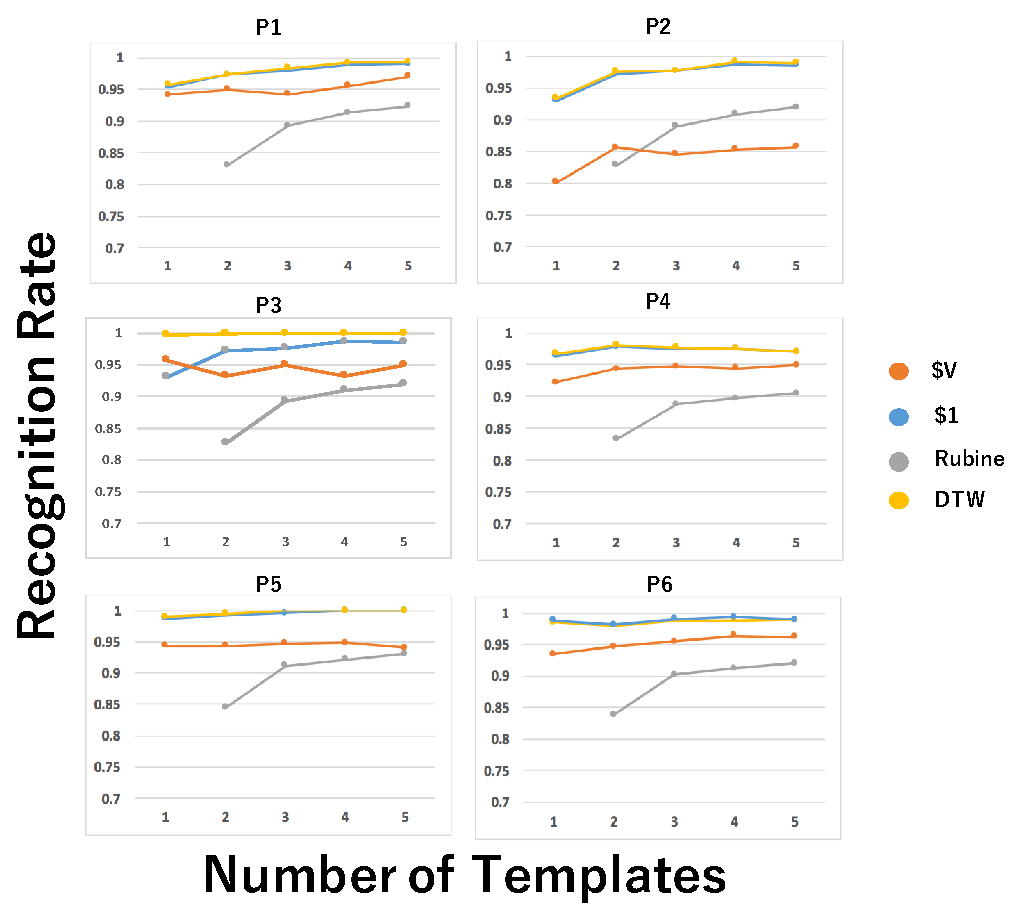
\includegraphics[width=1.0\columnwidth]{img/rec_rate.eps}
\caption{The screen shot on the smartphone. The green area is the input area}
\label{fig:rare_rec}
\end{figure}

それぞれの被験者の平均は,\$Vは93\%~(SD=4.55),\$1は98\%~(1.04),DTWは98\%~(0.86),Rubineは88\%~(2.14)であった.\$Vは\$1とDTWに対し,有意に低かった(p $<$ 0.01)が,被験者P1,P3,P4,P5,P6に関しては認識率の平均は95\%~(1.27)であり,\$1と比べて認識率の低下を最小限に抑えることに成功した.また,重み付けをしない場合と比べても,全被験者について認識率は向上した.
また,Rubineに対してP1,P3,P4,P5,P6に関しては有意に高かった(p $<$ 0.001).

P2の認識率が低かったのは,P2は別の名前のジェスチャで,似たような形状のジェスチャが複数存在したため,識別が困難になったことが要因であると考えられる.また,\$Vは学習データに比例して認識率が高くなるとは言えない.これは,同じジェスチャの学習データを追加するたびに,大きさ,向き,位置それぞれの特徴量を算術平均するため,必ずしも入力データに類似する学習データが存在する可能性が高くなるとは言えないからである.しかしながら,ほとんどの被験者において,少ない学習データにおいて高い認識率を示し,学習データが1つの場合における,全ジェスチャセットの認識率の平均は91.2\%(SD=0.07),学習データが2つの場合は92.2\%(0.04),学習データが3つの場合は92.7\%(0.05),学習データが4つの場合は93.3\%(0.04),学習データが5つの場合は93.2\%(0.05)となった.

\subsection{認識速度}
\subsection{\$V, \$1,Rubineの認識速度}
\begin{figure}[!h]
\centering
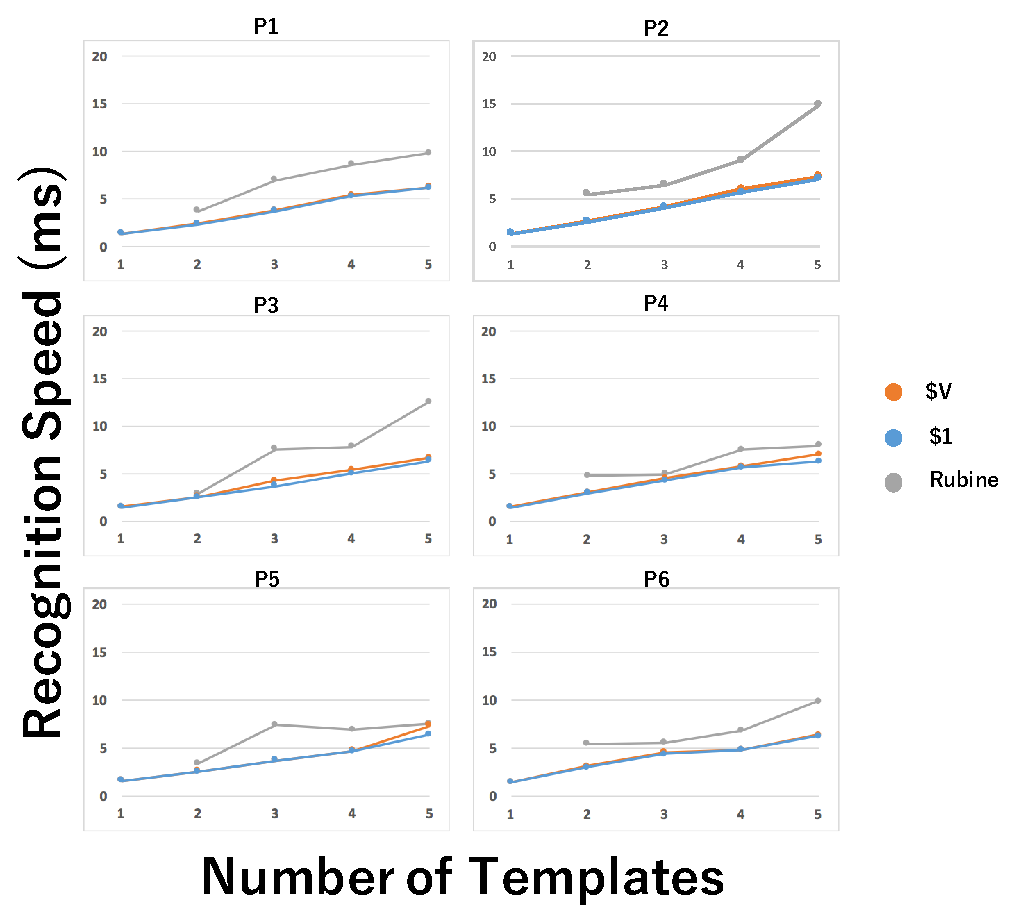
\includegraphics[width=1.0\columnwidth]{img/rec_speed.eps}
\caption{The screen shot on the smartphone. The green area is the input area}
\label{fig:rare_rec}
\end{figure}

\subsection{DTWの認識速度}
\begin{figure}[!h]
\centering
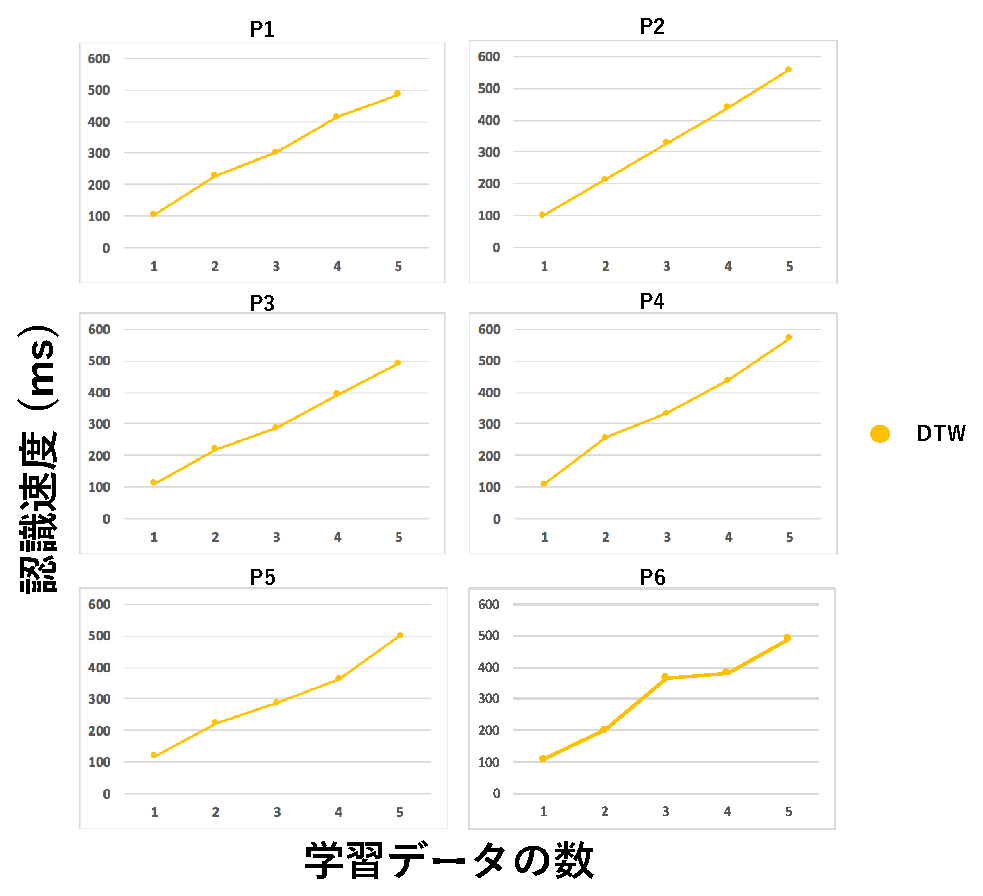
\includegraphics[width=1.0\columnwidth]{img/rec_speed_dtw.eps}
\caption{The screen shot on the smartphone. The green area is the input area}
\label{fig:rare_rec}
\end{figure}


\$Vの認識速度は,全被験者の平均が,学習データの数が1つの場合~2.6ms (SD=0.2),学習データの数が2つの場合~3.5ms (0.3),学習データの数が3つの場合~4.1ms (0.3),学習データの数が4つの場合~4.9ms (0.3),学習データの数が5つの場合~6.1ms (0.4)となり非常に速いと言える.また,\$1と認識速度に有意差はなく~(p $<$ 0.001),Rubineと比べると有意に速かった~(p $<$ 0.005).これらより,\$1と比べて認識速度の低下を抑えることに成功した.DTWの認識速度は図\ref{fig:rec_diff}に示すように非常に遅く,\$Vの認識速度はDTWのおよそ100分の1であった.
また,学習データに比例して認識速度が遅くなることも分かった.

\subsection{識別性能の結果}
\$Vの識別性能の結果を,N-best Listsの1番目と2番目の差及びジェスチャが一致した時の類似度及びジェスチャが一致した時の類似度の最小値を示すことによって述べる.

\subsubsection{N-best Listsの1番目と2番目の差}
\begin{figure}[!h]
\centering
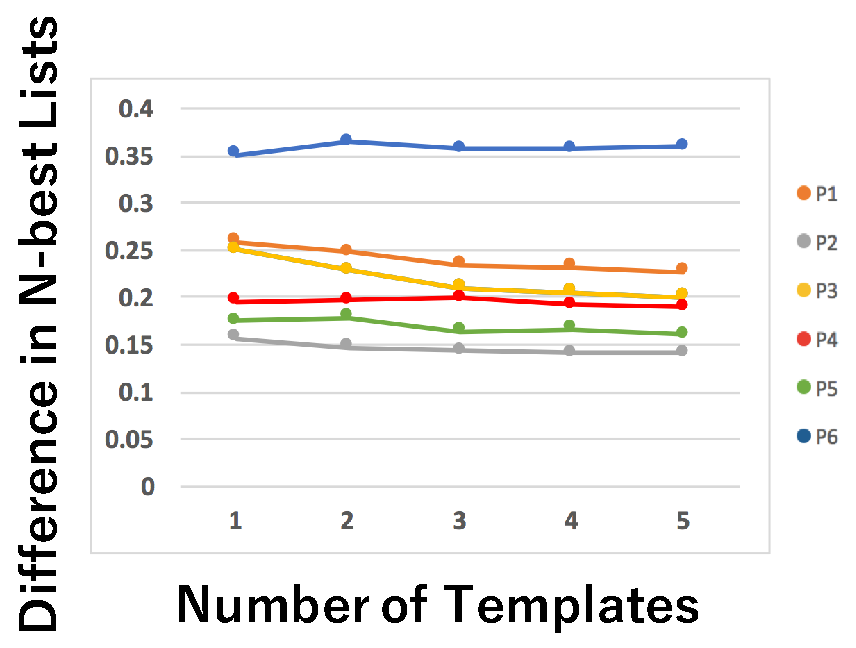
\includegraphics[width=0.7\columnwidth]{img/rec_diff.eps}
\caption{The screen shot on the smartphone. The green area is the input area}
\label{fig:rec_diff}
\end{figure}

\subsubsection{ジェスチャが一致した時の類似度}
\begin{figure}[!h]
\centering
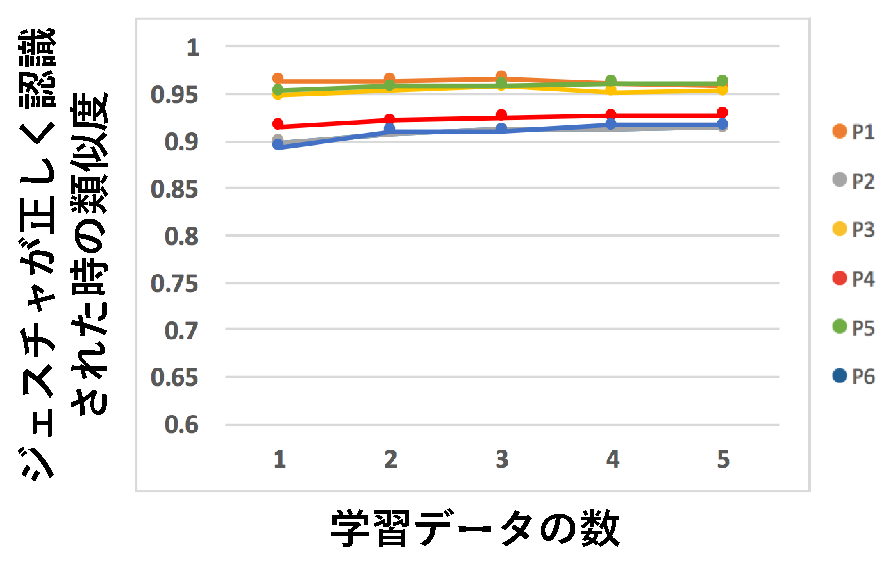
\includegraphics[width=0.7\columnwidth]{img/rec_sim.eps}
\caption{The screen shot on the smartphone. The green area is the input area}
\label{fig:rare_rec}
\end{figure}

\subsubsection{ジェスチャが一致した時の類似度の最小値}
\begin{figure}[!h]
\centering
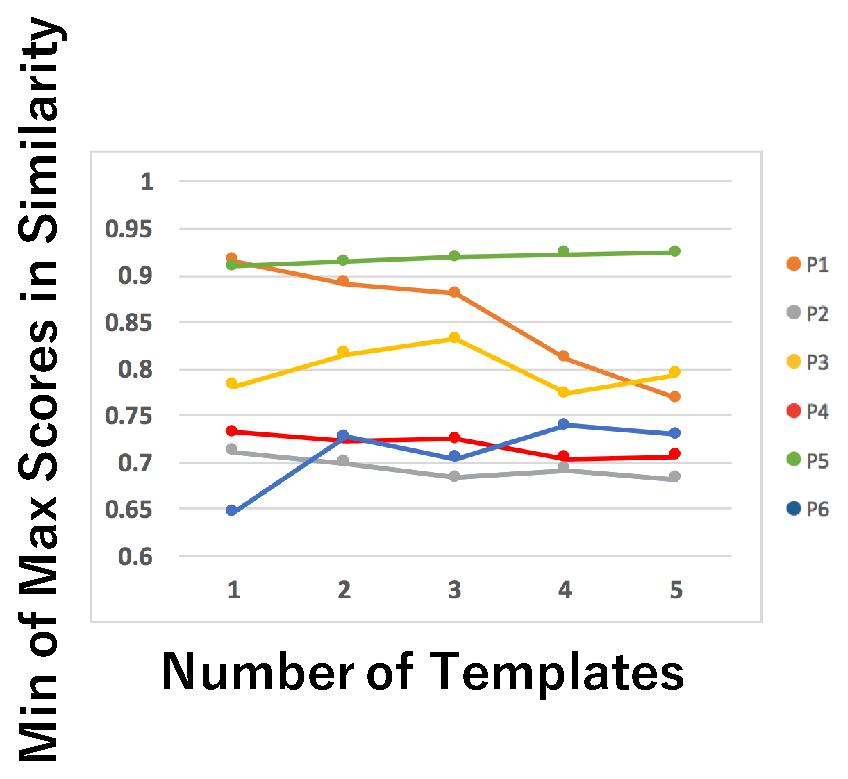
\includegraphics[width=0.7\columnwidth]{img/rec_min.eps}
\caption{The screen shot on the smartphone. The green area is the input area}
\label{fig:rare_rec}
\end{figure}

N-best Listsの1番目と2番目の差について,全ジェスチャセットの平均値はおよそ0.24~(SD = 0.1)となった.また,ジェスチャが一致した時の類似度の平均値は0.94~(SD=0.04)となり非常に高いと言えるが,ジェスチャが一致した時の類似度の最小値は被験者によってばらつきが生じ,平均値はおよそ0.83~(0.14)であった.また,N-best Listsの1番目と2番目の差は,重み付けをしない場合と比べて有意に高く~(p $<$ 0.01),識別性能が向上したと言える.しかしながら,ジェスチャが一致した時の類似度の最小値は,重み付けをしない場合と比べて有意に低かった~(p $<$ 0.01).これは,ジェスチャグループによっては,重み付けが最適でない場合があり,その場合類似度が低くなるからであると考えられる.よって,ジェスチャが一致した時の類似度の平均値が高いことから,重み付けは多くのジェスチャグループにおいて適用可能であるが,適用することによって類似度が低下する場合もあることがわかった.
また,ジェスチャが一致した時の類似度の最小値の平均はおよそ0.65以上であり,N-best Listsの1番目と2番目の差の平均値は0.15以上であることから,認識のための類似度の閾値を0.5とすることによって,ジェスチャが一致するか否かを判別することが可能となる.

以上を踏まえ,ジェスチャグループを作成し,ジェスチャグループ内に存在する学習データのみに対し,大きさ,向き,位置の類似度計算をすると認識速度の低下を防ぐことができるという仮説及び,同一ジェスチャグループ内において,他の学習データと類似している特徴量は,認識のための特徴量として用いなければ,認識率の低下を防ぐことができるという仮説は検証され,\$Vは.形状や書き順が同じ手書きジェスチャを大きさ,向き,位置に関して識別可能なアルゴリズムであると言える.

\TODO{学習データを追加する際の計算量を計測}
